\documentclass{mcmthesis}
\mcmsetup{CTeX = false,   % 使用 CTeX 套装时,设置为 true
        tcn = 72973, problem = B,
        sheet = true, titleinsheet = true, keywordsinsheet = true,
        titlepage = false}
\usepackage{palatino}
\usepackage{mwe}
\usepackage{graphicx}
\usepackage{subcaption}
\usepackage{amsmath}
\usepackage{float}
\usepackage{multirow}
\usepackage{indentfirst}
\usepackage{gensymb}
\usepackage[ruled,lined,commentsnumbered]{algorithm2e}
\usepackage{geometry}
\geometry{left=2cm,right=2cm,top=2cm,bottom=2cm}
\usepackage{booktabs}
\usepackage{mathrsfs}
\usepackage{esvect}
\usepackage{enumerate}
\newcommand{\RNum}[1]{\uppercase\expandafter{\romannumeral #1\relax}}


\begin{document}
\linespread{0.6}
\setlength{\parskip}{0.5\baselineskip}
\title{PTPs: E-Guide Helping Plan a Tour}%这里是标题

\date{\today}
\begin{abstract}
    When travelling in a new city, it is important but challenging to choose Points of Interests (POIs) to visit and design the route. The quality of a tour is highly dependent on tour planning. However, planning a tour takes much time and effort. \par
  To free the tourist from tour planning, our paper provides a personalized tour planning system (PTPs), which can offer the user a tour plan based on his/her preference, budget and time constraint. Moreover, we revise our PTPs to deal with ``super POIs'', namely, ones whose scale and structure can not be omitted. \par
  We first set up a criterion to characterize each POI's type and popularity. Then we build our PTPs model and examine its effectiveness by applying it to New York City (NYC).\par
  PTPs consists of three sub-models: Evaluation Model, Route Planning Model, and Hotel \& Restaurant Recommendation Model. There is a figure showing the connection between all parts.\par
  Evaluation Model gives each POI a ``satisfaction score''. It measures the closeness between the type of a POI and the user's preference, meanwhile considers the POI's popularity, and produce a score to describe how satisfactory a POI is for the user.\par
  Route Planning Model generates an optimal touring route under the constraints of time and budget. We apply a genetic algorithm to find a route with highest total satisfaction score. \par
  Hotel \& Restaurant Recommendation Model 

  To acquire the data we need, 
	\begin{keywords}
    tour planning, route design, 
	\end{keywords}
\end{abstract}

\maketitle
\tableofcontents

\newpage

\section{Introduction}	
\subsection{Background}
  Travelling to another city is a delightful experience for most people. There are so many places of interest to visit, such as museums, parks and so on. With limited time, tourists have to choose among those places and design their own route. Therefore, tour planning is a important task for tourists. However, it takes a lot of time and massive information to make a perfect plan, and several constraints(e.g. cost, transportation time, etc.) should be considered.
  \begin{figure}[ht]
    \centering
    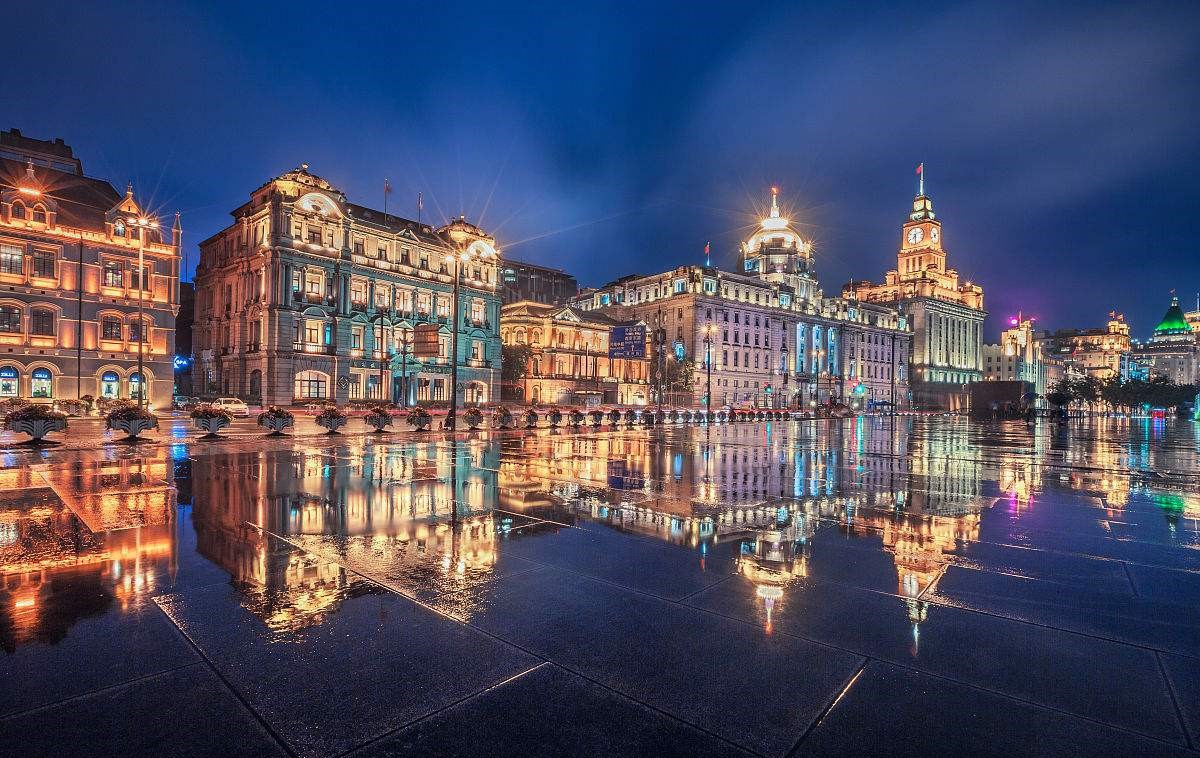
\includegraphics[width=\textwidth]{shanghai1.jpg}
    \caption{View of a city.}
    \label{fig:city}
  \end{figure}
\subsection{Restatement of problem}
  As required by the question, we are supposed to determine a tour route among Points of Interests (POIs), which include spots, hotels and restaurants. The route we provide should cover the popular POIs, meanwhile cater for the user's personal preference, namely, maximize the user's satisfaction, and meet the constraints. \par
  Furthermore, for ``super POIs'' (those with large scales) we should consider their inner structures, positions of entrances and exits and give a more subtle tour plan.
\subsection{Literature review}
  Existing study on tourism products recommendation applies one of the following four methods\cite{wen2014survey}:
  \begin{itemize}
    \item \textbf{Content-based recommendation,} which recommends tourism products similar to products chosen by the user.
    \item \textbf{Collaborative filtering recommendation,} which recommends the choice of users with similar preference.
    \item \textbf{Knowledge-based recommendation,} including constraint-based\cite{wang2012research} and case-based, makes recommendation according to Knowledge-based rules.
    \item \textbf{Social-based recommendation,} which applies users' relationship in social media.
  \end{itemize}
  Besides, in other works, factors such as distance\cite{Zhang2017GeoPMF}, user interests\cite{Qingxia2016Personalized}, and popularity\cite{li2016personalized} are taken into consideration. However, some of these methods are dependent on a large amount of historical datas, therefore have difficulties in cold-start. Moreover, datas on travelling are sparse, and getting these datas from users might be viewed as an invasion of privacy. \par
  There is also study on travelling route planning\cite{hao2015intellegent}. The majority of current works need users to input the origin and destination of travelling, and can not deal with accommodation arrangement, which limits their application. Therefore, we combine spot recommendation and route planning in our model, and get rid of reliance on historical datas.

  

\section{Assumptions}\label{section:assumption}
  To simplify the real life situation, we will make the following assumptions at the start of constructing our models.
  \begin{itemize}
    \item \textbf{Sightseeing is more important than accommodation.} User's preference of spots are considered in higher priority than restaurants and hotels. 
    \item \textbf{We further assume that a tourist always stays in the same hotel during a trip.} The user doesn't have to bother carrying.
    \item \textbf{User's satisfaction on POIs solely depends on his/her preference and the popularity,} while the impact of other factors(e.g. mood, weather, etc.) is neglected. Because the quality of POIs is vague and subjective, thus hard to quantitify, we assume that generally the more popular a POI is, the higher quality it is of.
    \item \textbf{Road between any two spots is straight, and its length is approximately equal to the great-circle distance.}
    \item \textbf{Ticket and traffic fares are ignorable compared to prices of hotels and restaurants.} Therefore, the cost of visiting a spot and travelling between spots can be viewed as zero.
    \item \textbf{The spots' scales are relatively small,} including super POIs. In the scale of the city, a super POI can still be viewed as a point. In the scale of a super POI, the subspots in it can be viewed as points. Therefore, the time taken moving from one spot to another within a super POI is ignorable.
  \end{itemize}


\section{Nomenclature}
  \begin{tabular}{lll}    %记号表
    \toprule
    Notation & Definition & Unit \\
    \midrule
    $\vv{cat}$ & Vector that describes a spot's category & \\
    $\vv{prf}$ & Vector that describes the user's preference of spots' category & \\
    $Intr$ & Rate of user's interest to a certain spot & \\
    $Pop$ & Rate of POI's popularity among the public & \\
    $Sat$ & Score of satisfaction of a spot & \\
    $t_{dur}$ & Time duration of touring in a spot & hour \\
    $t_{tra}$ & Time duration of traffic between two spots & hour \\
    \bottomrule
  \end{tabular}


\section{Model \RNum{1}: Personalized Tour Planning System (PTPs)} \label{section:model1}
  In this section, we will discuss our models. Before diving into details, briefly explain the whole idea (as figure \ref{fig:model} shows). Firstly, we give each spot a score based on its popularity and closeness to user's preference. Then we construct a graph, containing scores, traffic time and tour duration. We apply a genetic algorithm to find a way maximizing the score under the constraints of time. Furthermore, we analysis the relation between final satisfaction score and some properties.
  \begin{figure}[ht]
    \centering
    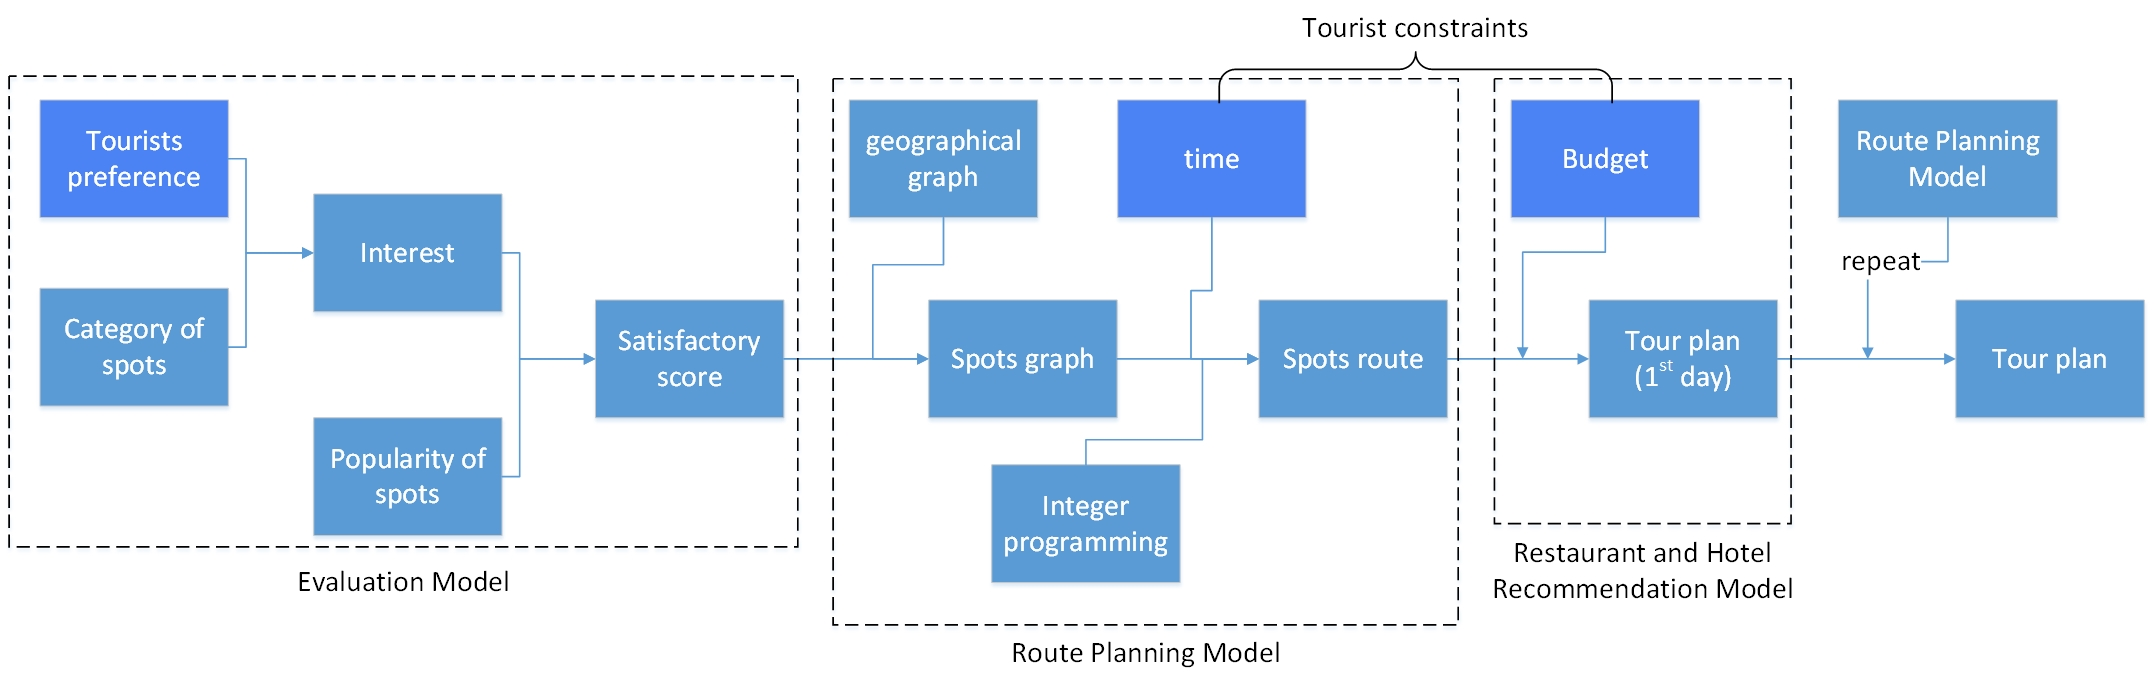
\includegraphics[width=\textwidth]{model.jpg}
    \caption{Overview of Personalized Tour Planning System}
    \label{fig:model}
  \end{figure}
\subsection{Rate the POIs: Evaluation Model}
  We define a series of dimensions to classify the POIs(e.g. landmark, museum, historical site, etc.) A spot is assigned a value ranging from 0 to 1 for each dimension. Thus we build a category vector $\vv{cat} = [r_{1}, r_{2}, \ldots, r_{n}]$, where $r_{i}$ denotes the rate of $i^{th}$ category, to classify each spot. Through a user inerface, the user is asked to input the following values:
  \begin{itemize}
    \item His/her ``interest rate'' to each category of POI;
    \item Total travelling time limit;
    \item Highest budget acceptable.
  \end{itemize}
  We normalize the data, thus getting the user's preference vector $\vv{prf}$, which is a unit vector. Then the rate of user's interest to a certain spot() can be calculated: 
  \[
    Intr(s1) = cos<\vv{cat}(s1),\vv{prf}>
  \]
  To quantitify the each POI's popularity $Pop$, we acquire the datas of search volume and rating. We normalize the datas using a linear mapping, in which the maximum and minimum are converted to 1 and 0, respectively. Then we calculate the POI's satisfaction score by the following fomula:
  \[
    Sat = \alpha Intr + (1-\alpha)Pop
  \]
  where $\alpha$ is a positive weighting coefficient.

\subsection{Construction of the graph}
  \paragraph{Data acquirement} \

  After giving each POI a score, we calculate the distance between each two POIs by their latitudes and longitudes using Haversine fomula:
  \[
    hav(\frac{d}{r}) = hav(\varphi_{2}-\varphi_{1}) + cos(\varphi_{1})cos(\varphi_{2})hav(\lambda_{2}-\lambda_{1})
  \]
  where:
  \begin{itemize}
    \item $hav$ is the haversine function: $hav(\theta) = sin^{2}(\frac{\theta}{2})$;
    \item $d$ is the distance between two spots along the great circle of the sphere;
    \item $r$ is the radius of the sphere, namely the radius of earth in this case;
    \item $\varphi$ and $\lambda$ represent the latitude and longitude respectively.
  \end{itemize} 
  We estimate the speed of each kind of transportation, and with the distance between spots $d$ assigned, we can calculate the traffic time taken between each two spots. \par
  \paragraph{Construct the graph} 

  With the datas prepared, we construct a weighted directed graph (figure \ref{fig:graph}), of which the nodes are spots. Every node is weighted by its score, and has touring duration as another property. The edge, which denotes road between the two spots it connects, is weighted by the traffic time.
  \begin{figure}[ht]
    \centering
    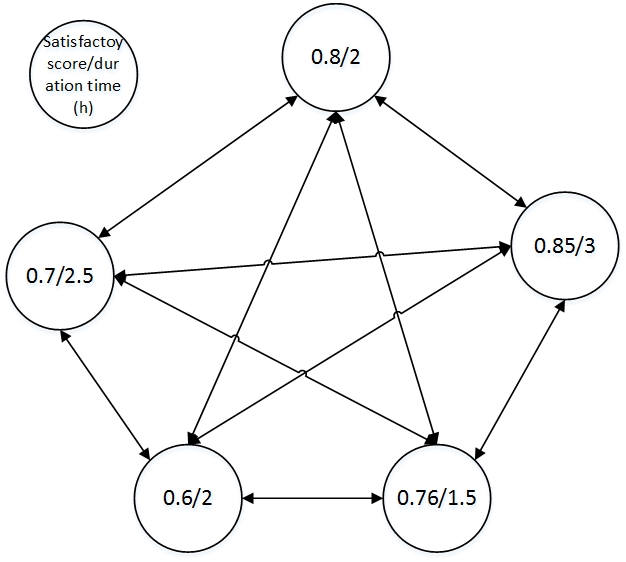
\includegraphics[width=0.6\textwidth]{graph.jpg}
    \caption{Structure of Weighted Graph Model}
    \label{fig:graph}
  \end{figure}

%%%%%%%%%%%GA===================================================================================================================
\subsection{Plan the Tour Route}
  With all the spots rated and a weighted graph constructed, we apply a genetic algorithm (as figure \ref{fig:ga} shows) with non-linear constraints to generate a near-optimal route:
  \begin{alignat}{2}   %遗传算法
    \max~\sum_{i=1}^{n}Sat(s_{i})~(fitness function)\\
    \mbox{s.t.}\quad
    &\sum_{i=1}^{n}t_{dur}(s_{i}) < t_{max}\\
    &s_{i}~is~only~toured~one~time, & (i=1,2,\ldots,n)
  \end{alignat}
  where:
  \begin{itemize}
    \item $s_{i}$ is the $i^{th}$ spot, $i=1,2,\ldots,n$, $n$ is the total amount of spots;
    \item $t_{max}$ is the longest total travelling time duration that the tourist can accept.
  \end{itemize}
  \begin{figure}[ht]
    \centering
    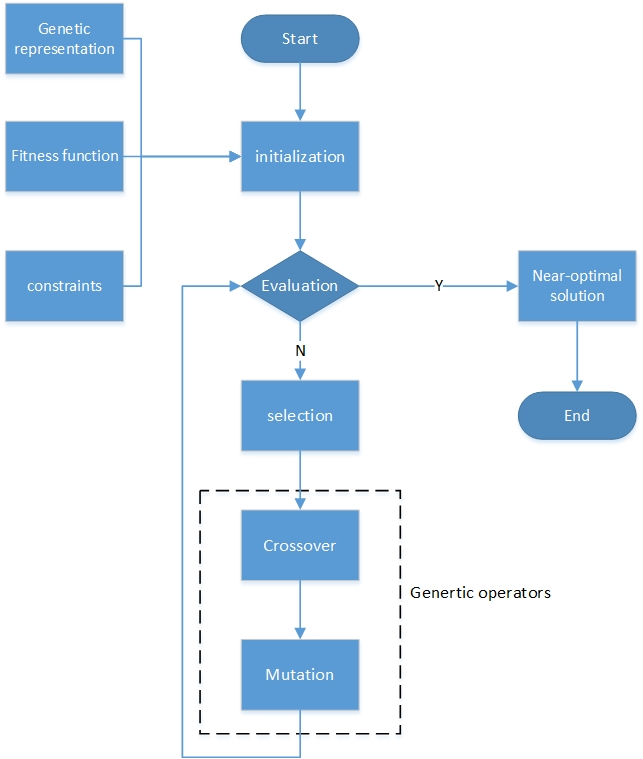
\includegraphics[width=0.6\textwidth]{ga.jpg}
    \caption{Sketch of genetic algorithm}
    \label{fig:ga}
  \end{figure}
  we use path coding method, represent a path starting from spot $s_{k0}$ via $s_{k1}, s_{k2},\ldots,s_{km}$ with $k0-k1-\cdots-km$. Applying the \emph{ga} funtion in MATLAB, we find out a near-optimal route and the corresponding value of fitness function.
  %To find out the optimal tour route is an OP problem\cite{Gionis2014Customized}. We first set the spot with highest score as the origin and destination of all routes, and generate all possible routes which suit the constraint of time. Then, for each potential route, we sum up the scores of all spots it contains, thus the routs are rated. The route scoring highest is chosen as the recommended route for the first day. For other days, the same operation is applied among spots the user hasn't been to. 

  



\subsection{Restaurant \& Hotel Recommendation}
  After providing a route to travel around spots, we work on ways to recommend hotels and restaurant to consummate our tour planning system. Since hotels and restaurants are different in many ways, we use different methods in recommendation.
  \paragraph{Restaurants}\
  
  From the route planning process, a travelling sequence $\mathscr{S} = [s_{1}, s_{2}, \ldots, s_{n}]$ is generated. We can also generate a sequence of starting times and ending times of touring the spots, $\mathscr{T} = [t_{1}, t_{2}, \ldots, t_{2n}]$. If we set a meal time(e.g. 12am for lunch and 6pm for supper), we can find a $t_{m}$ in $\mathscr{T}$ that is closest to the meal time, and find the corresponding $s_{k}$ of $t_{m}$. \par
  Then we seek for restaurants that suits the constraints in a circle with $s_{k}$ as center and a radius of 500 meters (might be adjusted due to the user's preference). With the similar method we apply in rating the spots, we give each restaurant a score according to its category, popularity and the user's preference. The one with highest score is what we recommend to the user.
  \paragraph{Hotels}\
  
  As stated in \ref{section:assumption}, the tourist stay in the same hotel during the whole tour. In our model, we first list the spots in the first day's schedule, and select from the hotels economically suitable in a 500m-radius-circle around each spot. The hotel with best popularity among those selected ones will be our recommendation.

\section{Model \RNum{2}: PTPs with Super POIs} \label{section:model2}
  In \ref{section:model1}, we regard the POIs as points without shape, inner structure and volume. For the Super POIs, inner information should be take into consideration, therefore we revise our model (figure \ref{fig:model2}). To begin with, we evaluate the POIs and generate a optimal route using PTPs model. Then we transform each super POI to a weighted graph, in which the nodes are gates and subspots to view. Each subspot has a tour duration as its property. \par
  \begin{figure}[ht]
    \centering
    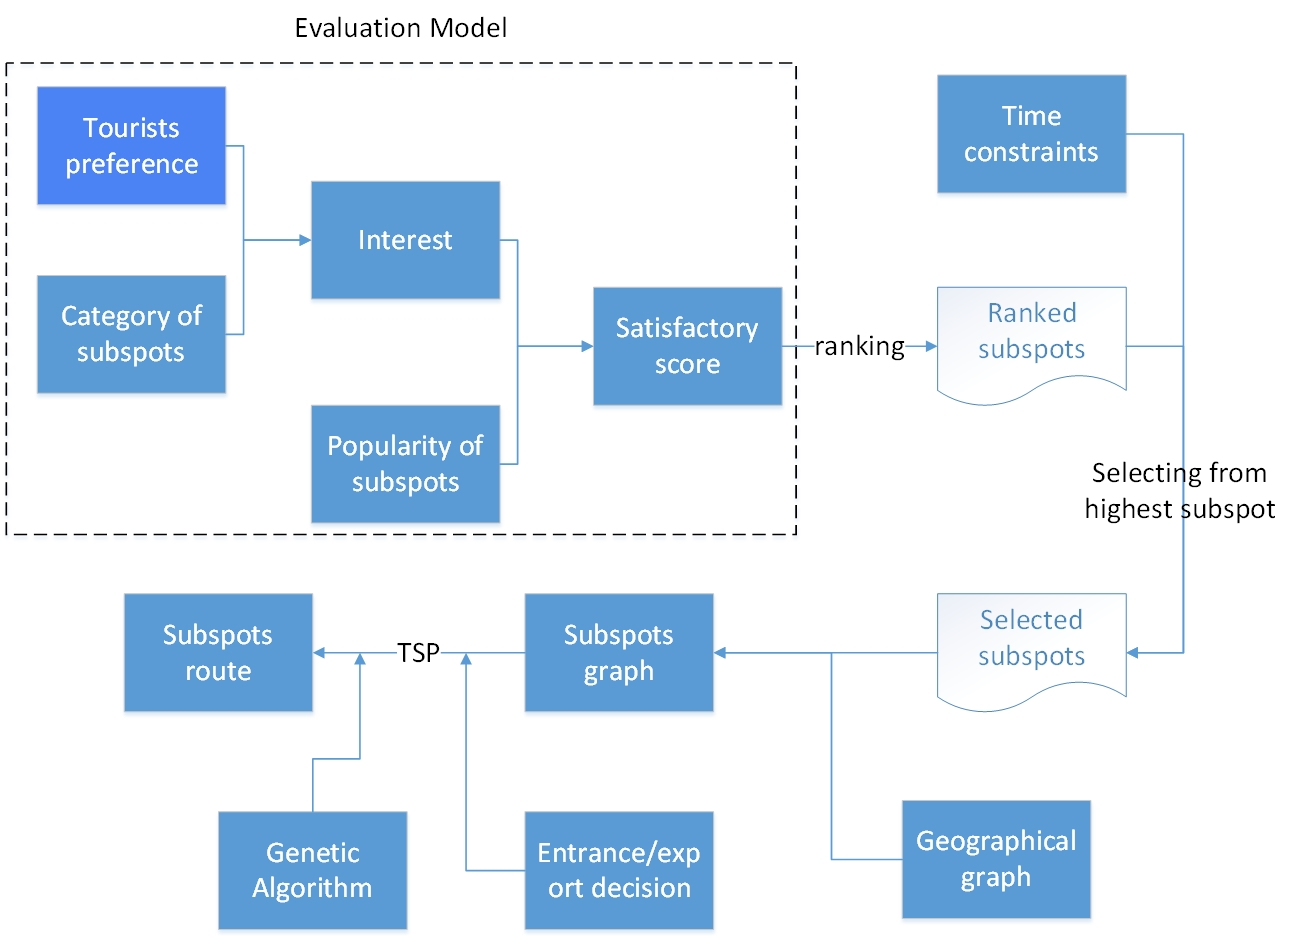
\includegraphics[width=\textwidth]{model2.jpg}
    \caption{Overview of the revised model}
    \label{fig:model2}
  \end{figure}
  In the tour route generated, each super POI has two adjacent nodes (two spots). We select two gates with least distance to the adjacent nodes and decide the entrance and exit according to the tour direction. After the selection of gates is done, we design the tour route inside the super POI. Using the evaluation model we give each subspot a satisfaction score. And because the traffic time between subspots is ignorable, we just need to maximize the total satisfaction score under the constraint of time. \par
  To choose among all subspots in a super POI, we apply a greedy algorithm: Pick the highest-scored subspot, and then pick the highest-scored one from the left ones $\cdots$ until total tour duration reaches the time limit. Planning a route to tour around the chosen subspots starting from the entrance and ending at the exit is a travelling salesman problem (TSP).




\section{Inplementation}
  To test our PTPs model, we first apply it to New York City (NYC). Using the information we gathered, we apply the models and design a tour plan in NYC.
\subsection{Data}
  Because there is no existing dataset about NYC's POIs, in this paper we ourselves analyze many datas from reliable sources and experiment with them. We acquire a list of POIs in NYC from the \emph{Trip Advisor} website\cite{TripAdv}. Then we gather detailed information from Google's Places API Web Service\cite{GMaps}, including:
  \begin{itemize}
    \item The position of each POI, namely its latitude and longitude.
    \item The ticket price of each POI;
    \item Search volume and public rate of each POI.
  \end{itemize}
  Applying the methods mentioned in \ref{section:model1}, we get the distance between each two POIs in NYC, and each spot's price and satisfaction score. 
\subsection{Analysis \& Results}
  \paragraph{Tour plan} \
  
  We simulate some ``users'' and input their requests (available time, preference of POIs, etc.) to our PTPs and generate personalized tour plans for them. 
  \paragraph{Analysis of result} \
  
  To examine the effectiveness of our PTPs, for each ``user'' we generate a series of alternative tour plans using a randomized algorithm. We calculate the total satisfaction score for each tour plan, including the PTPs-recommended one and the randomized ones. We find out that the tour plan PTPs generates has great advantages in comparison to other plans, that is to say, has the highest satisfaction score among the plans. \par
  For further discussion, we calculate the satisfaction scores (fitness values) under different $t_{max}$, and visualize the result in figure \ref{fig:sstt}.
  \begin{figure}[ht]
    \centering
    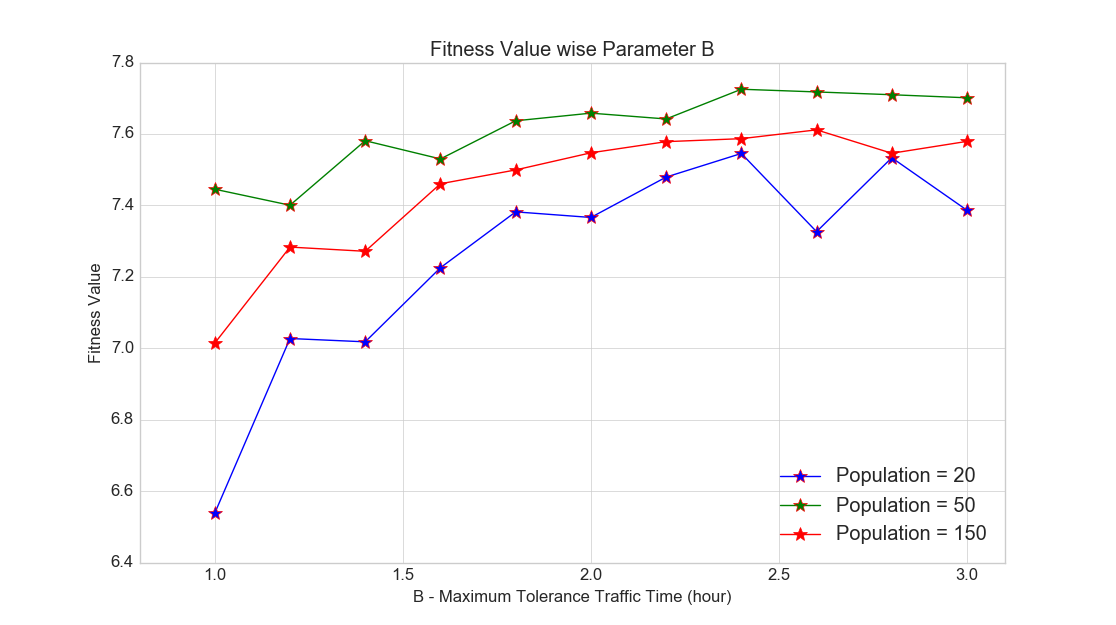
\includegraphics[width=\textwidth]{popularity.png}
    \caption{Relationship between satisfaction score and traffic time limit.}
    \label{fig:sstt}
  \end{figure}




\section{Model Analysis}
\subsection{Sensitivity Analysis}

\subsection{Strengths \& Weaknesses}
\subsubsection{Strengths}
  \begin{enumerate}
    \item Have the ability of cold-start. Our model can give personalized tour plan without the user's historical data.
    \item Combine the processes of choosing which POIs to go and designing the route in one app/website.
    \item Use massive accurate data of New York City. Only with these dependable data can we validate that our model is built appropriately.
    \item 
  \end{enumerate}
\subsubsection{Weaknesses}
  \begin{enumerate}
    \item Complex traffic conditions in cities are omitted. We simplify the traffic network to weighted graph. However, in the real condition there are much more factors influencing the traffic time.
    \item Tourist's satisfaction is assumed only related to his/her interest and the POI's popularity. The impact of complex subjective and emotional factors during the tour are not considered.
    \item 
  \end{enumerate}

\section{Conclusion}





\bibliographystyle{IEEEtran}
\bibliography{newrefs}

\newpage
\section*{Get FREE from Tour Planning!}
  \begin{figure}[ht]
    \centering
    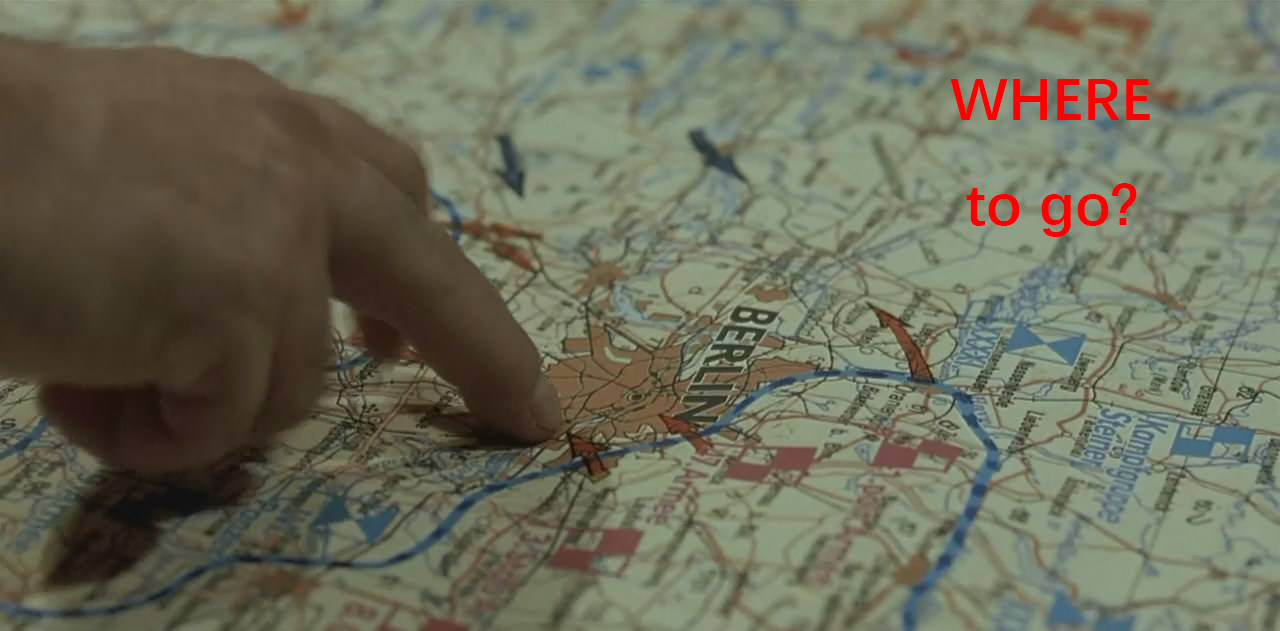
\includegraphics[width=\textwidth]{ad.png}
  \end{figure}
Want to explore a new city? Hard to decide where to go? \par
Ooooh, a tour should be relaxed. Don't let tour planning burden you! \par
  \centering
Why not experience the convenience \emph{Where to GO} provides!\par
  \begin{figure}[ht]
    \centering
    
\includegraphics[width=\textwidth]{cwg.png}
  \end{figure}
\begin{large}
  Personalized tour planning, a touch and all done.
\end{large}

	

	
\newpage

\begin{appendices}

\end{appendices}





\end{document}